\input{/Users/daniel/github/config/preamble.sty}%available at github.com/danimalabares/config
\input{/Users/daniel/github/config/thms-eng.sty}%available at github.com/danimalabares/config


\usepackage[style=authortitle-terse,backend=bibtex]{biblatex}
\addbibresource{bibliography.bib}

\setcounter{secnumdepth}{2}

\begin{document}

\begin{minipage}{\textwidth}
	\begin{minipage}{1\textwidth}
		K3 surfaces \hfill Daniel González Casanova Azuela
		
		{\small Prof. Misha Verbitsky\hfill\href{https://github.com/danimalabares/k3}{github.com/danimalabares/k3}}
	\end{minipage}
\end{minipage}\vspace{.2cm}\hrule

\vspace{10pt}
{\huge Home assignment 6: cohomology and intersection forms}

\begin{thing1}{Exercise 6.1}\leavevmode
	Compute the cohomology algebra of the manifold
	\begin{enumerate}[label=\alph*.]
		\item $\mathbb{C}P^{2}\#\mathbb{C}P^{2}$
		\item $\mathbb{C}P^{2}\#\overline{\mathbb{C}P^{2}}$ 
		\item $(S^2\times S^3)\#(S^2\times S^3)$
		\item $\mathbb{H}P^2$
	\end{enumerate}
\end{thing1}

\begin{proof}[Solution]\leavevmode
	\begin{enumerate}[label=\alph*.]
		\item First let's compute the cohomology groups. After several attempts I will use the following simple argument from \href{https://math.stackexchange.com/questions/3635669/cup-products-in-cohomologies-of-connected-sum-of-copies-of-a-specific-manifold}{StackExchange}.  Recall that the connected sum is obtained by removing a 4-dimensional disk in $\mathbb{C}P^{2}$ and glung another copy of $\mathbb{C}P^{2}$ along the boundary $S^3$ of the removed disk.This makes $(\mathbb{C}P^{2}\#\mathbb{C}P^{2},S^3)$ a \textit{\textbf{good pair}} ($S^3$ is a deformation retract some open neighbourhood in $\mathbb{C}P^{2}\#\mathbb{C}P^{2}$). This means that relative cohomology may be identified with the homology of the quotient:
			\[H_{\bullet}(\mathbb{C}P^2\#\mathbb{C}P^2,S^3)=H_{\bullet}(\mathbb{C}P^2\#\mathbb{C}P^2/S^3)=H_{\bullet}(\mathbb{C}P^2\vee\mathbb{C}P^2)=H_{\bullet}(\mathbb{C}P^{2})\oplus H_\bullet(\mathbb{C}P^{2})\]
			And then we have the long sequence for relative homology, which may be written more succintly as
			\[\begin{tikzcd}H_{\bullet}(\mathbb{C}P^{2})\oplus H_\bullet(\mathbb{C}P^{2})\arrow[r]& H_\bullet(\mathbb{C}P^{2}\#\mathbb{C}P^{2})\arrow[r]&H_\bullet(S^3)\end{tikzcd}\]
			Which gives by Poincaré duality
			\[H^{0}(\mathbb{C}P^2\#\mathbb{C}P^2)=H^{4}(\mathbb{C}P^2\#\mathbb{C}P^2)=\mathbb{Z}\]
			This is because $\mathbb{C}P^{2}\#\mathbb{C}P^{2}$ is connected; there is no isomorphism $H_{\bullet}(\mathbb{C}P^{2})\oplus H_\bullet(\mathbb{C}P^{2})=\mathbb{C}P^2\#\mathbb{C}P^2$ because it is the first/last terms of the sequence, where $H^{\bullet}(S^3)$ does not vanish. For the other terms there \textit{is} an isomorphism because the homology of the sphere vanishes:
			\[H^{i}(\mathbb{C}P^2\#\mathbb{C}P^2)=H^{i}(\mathbb{C}P^{2})\oplus H^{i}(\mathbb{C}P^{2}),\qquad i=1,2,3\]
			which means that
			\[H^{i}(\mathbb{C}P^2\#\mathbb{C}P^2)=0,\qquad i=1,3\]
			\[H^{2}(\mathbb{C}P^2\#\mathbb{C}P^2)=\mathbb{Z}\oplus \mathbb{Z}\]
In the \href{https://math.stackexchange.com/questions/3635669/cup-products-in-cohomologies-of-connected-sum-of-copies-of-a-specific-manifold}{StackExchange} answer I'm using it is claimed that the product structure should be given by 
\begin{align*}
	\smile\;: \underbrace{H^{2}(\mathbb{C}P^2\#\mathbb{C}P^2)}_{H^{2}(\mathbb{C}P^{2})\oplus H^{2}(\mathbb{C}P^{2})}\times \underbrace{H^{2}(\mathbb{C}P^2\#\mathbb{C}P^2)}_{H^{2}(\mathbb{C}P^{2})\oplus H^{2}(\mathbb{C}P^{2})} &\longrightarrow H^{4}(\mathbb{C}P^2\#\mathbb{C}P^2) \\
	\Big((\alpha,\beta),(\alpha',\beta')\Big)\qquad \qquad  &\longmapsto \alpha\smile\alpha'+\beta\smile\beta'
\end{align*}
but I cannot see why.



			\iffalse This is done via Mayer-Vietoris. Recall that the connected sum is obtained by removing a 4-dimensional disk in $\mathbb{C}P^{2}$ and glung another copy of $\mathbb{C}P^{2}$ along the boundary $S^3$ of the removed disk. To apply Mayer-Vietoris consider a neighbourhood for every copy of $\mathbb{C}P^{2}$, each containing the whole copy of $\mathbb{C}P^{2}$ a small part of the other copy in such way the two neighbourhoods intersect in an open set (see figure).
			\begin{figure}[H]
				\centering
				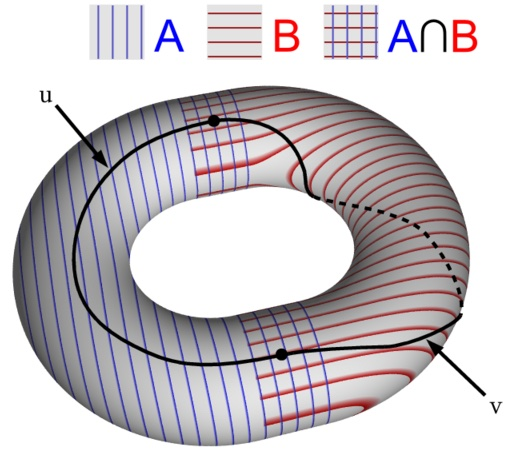
\includegraphics[width=0.3\textwidth]{fig1}
				\caption{An open cover for Mayer-Vietoris for torus\\ (ignore the curve and labels \textbf{u}, \textbf{v}).  }
			\end{figure}
			Calling $X=\mathbb{C}P^{2}\#\mathbb{C}P^{2}$ and the two neighbourhoods $A $ and $B$, we get the exact sequence
			\[\begin{tikzcd}[column sep=small]
			0\arrow[r]&H^{0}(X)\arrow[r]&H^{0}(A)\oplus H^{0}(B)\arrow[r]&\cancelto{0}{H^{0}(S^3)}\arrow[r]&\leavevmode
			\end{tikzcd}\]

			\[\begin{tikzcd}[column sep=small]
			0\arrow[r]&	\cancelto{\mathbb{Z}}{H^{0}(S^3)}\arrow[r,"\cong "]&H^{1}(X)\arrow[r]&\cancelto{0}{H^{1}(A)\oplus H^{1}(B)}\arrow[r]&\cancelto{0}{H^{1}(S^3)}\arrow[r]&\leavevmode
			\end{tikzcd}\]
			\[\begin{tikzcd}[column sep=small]
				\leavevmode\arrow[r]&H^{2}(X)\arrow[r,"\cong "]&H^{2}(A)\oplus H^{2}(B)\arrow[r]&\cancelto{0}{H^{2}(S^3)}\arrow[r]&H^{3}(X)\arrow[r]&\cancelto{0}{H^{3}(A)\oplus H^{3}(B)}\arrow[r]&\leavevmode			\end{tikzcd}\]
				\[\begin{tikzcd}[column sep=small]
			\arrow[r]&\cancelto{\mathbb{Z}}{H^{3}(S^3)}\arrow[r]&H^{4}(X)\arrow[r,"\cong "]&H^{4}(A)\oplus H^{4}(B)\arrow[r]&0
				\end{tikzcd}\]
				where the cohomology of $A $ and $ B$ equals the cohomology of $\mathbb{C}P^{2}$ in degrees $<4$. This is a general fact:

				\begin{claim}\leavevmode
					(See \href{https://math.stackexchange.com/questions/4816763/intuition-for-killing-homology-group}{StackExchange}.) If a space $\tilde{Y}$ obtained from $\tilde{X}$ by attaching a ($n+1$)-cell then their homology is the same in degree $<n+1$.
				\end{claim} 
				\begin{proof}[Proof of claim]\leavevmode
					Notice the 
				\iffalse\textit{\textbf{characteristic map}} $\Phi:D^{n+1}\to \tilde{X}$ that gives
				\[\tilde{Y}=(D^{n+1}\sqcup \tilde{X})\Big/\sim ,\qquad \text{where } x \sim \Phi(x)\text{ for }x\in\partial D^{n+1} \]
				Indeed, $\Phi$ is a map of pairs $(D^{n+1},S^n)\to (\tilde{Y},\tilde{X})$ that induces an
				\fi isomorphisms of relative homology
				\[H_k(D^{k+1},S^k)\cong H_k(\tilde{Y},\tilde{X})\qquad \text{ for all $k$.} \]
				These hold because if  $\tilde{X}$ and $\tilde{Y}$ are a good pair ($\tilde{X}$ is a deformation retract some open neighbourhood in $\tilde{Y}$), relative homology equals homology of the quotient, i.e. \[H_k(D^{k+1},S^k)\cong H_k(D^{k+1}/S^k)\qquad \text{and}\qquad  H_k(\tilde{Y}/\tilde{X})=H_k(\tilde{Y},\tilde{X})\]
				And the spaces $D^{k+1}/S^k$ and  $\tilde{Y}/\tilde{X}$ are homotopic since all that is left of  $\tilde{Y}$ after collapsing $\tilde{X}$ coincides with what is left of $D^{k+1}$ after collapsing $S^k$. Then, from the relative homology exact sequence
\[\begin{tikzcd}[column sep=small]
	\cdots\arrow[r]&H_{k}(\tilde{Y})\arrow[r]&H_k(\tilde{X})\arrow[r]&H_k(\tilde{Y},\tilde{X})\arrow[r]&H_{k-1}(\tilde{Y})\arrow[r]&\cdots
\end{tikzcd}\]
				we see that $H_k(\tilde{X})\cong H_k(\tilde{Y})$ for $k<n+1$.
\end{proof}
				We apply this to our exercise since $\mathbb{C}P^{2}$ is obtained from $A=B$ by attaching a 4-cell. Knowing the cohomology of $A=B$ we use the Mayer-Vietoris sequence and Poincaré duality we have that
			\[H^{1}(\mathbb{C}P^{2}\#\mathbb{C}P^{2})\cong0\cong H^{3}(\mathbb{C}P^{2}\#\mathbb{C}P^{2})\qquad \text{ and } \qquad H^{2}(\mathbb{C}P^{2}\#\mathbb{C}P^{2})\cong\mathbb{Z}\oplus \mathbb{Z}.\]
				\iffalse

				\begin{itemize}
\item the cohomology of $A$ and $B$ in degree 3 must equal degree 1-homology by Poincaré duality, and the latter vanishes since otherwise it would equal the abelizanization of the fundamental group, which is trivial in $\mathbb{C}P^{2}$ and remains unaffected after the removal of a 4-ball.

\item the cohomology of $A$ and $B$ in degree 1 must equal degree 3 homology by Poincaré duality as well, and in this case vanishes because $A$ and  $B$ have a CW structure with one 0-cell, one 2-cell, one 3-cell (the boundary of the removed 4-ball) and one 4-cell.

\item the cohomology of $A$ and $B$ in degree 2
\end{itemize}

				, yielding $H^{2}(A)=H^{2}(B)=H^{2}(\mathbb{C}P^{2})=\mathbb{Z}$, so
				\[H^{2}(X)\cong \mathbb{Z}\oplus \mathbb{Z}.\]\fi
			To compute degree 4 cohomology of $A$ and  $B$ we look at the relative sequence of homology in degree 0:			\[\begin{tikzcd}[column sep=small]
				\underbrace{H^0(\mathbb{C}P^{2},A)}_{\cong H^0(S^3)\cong 0}\arrow[r]&H_0(A)\arrow[r]&\underbrace{H_0(\mathbb{C}P^{2})}_{\cong\mathbb{Z}}\arrow[r]&\underbrace{H_0(\mathbb{C}P^{2},A)}_{\cong H_0(S^3)\cong\mathbb{Z}}\arrow[r]&0\arrow[r]&\cdots
			\end{tikzcd}\]
			And since this sequence splits (because the group in the right-hand side is free, see Hatcher p. 148), meaning that $H_0(A)\cong H^{4}(A)\cong 0$, so that
			\[H^{4}(\mathbb{C}P^{2}\#\mathbb{C}P^{2})\cong 0\]

			We still need to compute the ring structure.

			\end{enumerate}
\end{proof}

\begin{thing7}{Exercise 6.6}\leavevmode
	Define the blow-up of a complex manifold in a point, and prove that the blow-up of $\mathbb{C}P^{n}$ in a point is diffeomorphic to $\mathbb{C}P^{n}\#\overline{\mathbb{C}P^{n}}$.
\end{thing7}

\begin{proof}[Solution]\leavevmode
	Let's see what I remember of blow-up. The \textit{\textbf{blow-up}} of the complex plane at the origin is the variety obtained by substituing the point 0 with $\mathbb{C}P^{1}$. It has associated some equations that go something like
	\[u_iv_j=u_jv_i\]
	And then this gives a covering map
	\[\begin{tikzcd}
	\operatorname{Bl}_0\mathbb{C}\arrow[d,"\pi"]\\
	\mathbb{C}
	\end{tikzcd}\]
	and the fiber of 0, which is $\mathbb{C}P^{1}$, is called the \textit{\textbf{exeptional divisor}}. So according to all I've recently learnt  about divisor then $\mathbb{C}P^{1}$ should be a divisor of $\operatorname{Bl}_0\mathbb{C}$ that is of course exeptional in the sense that all other divisors are just points and that one is a 1-dimensional variety.

	And that's pretty much all I can say. I think the blow-up can be generalized to any subvariety of any variety giving $\operatorname{Bl}_YX$ but that means what? Substituting the variety with some projective variety?

	Anyway here I want to blow-up only a point in $\mathbb{C}P^{n}$. So I think this will be putting $\mathbb{C}P^{1}$ instead of the point. Now to show that this is connected sum… Mmm intuitively… but take the case of $ \mathbb{C}$: how do you glue $\mathbb{C}P^{1}$ at 0? $\mathsf{OK}$ let's see Hartshorne.
\fi
		\begin{remark}\leavevmode
				In \href{https://www.math.stonybrook.edu/~milivojevic/model2cp2.pdf}{this document} it is claimed (using \textit{\textbf{formal manifolds}}) without proof that
				\begin{quotation}
					To obtain the cohomology algebra of a connect sum, tensor the cohomology algebras of the spaces you are connecting, and impose the relations that all products of elements coming from different connect-summands are zero, and identify the volume forms. […] So, the cohomology algebra of the connect sum of $\mathbb{C}P^{2}$ is
				\begin{align*}H^{\bullet}(\mathbb{C}P^{2}\#\mathbb{C}P^{2})=\Lambda(a,b;&\operatorname{deg}(a)=\operatorname{deg}(b)=2,a^3=0,\\&b^3=0,ab=0,a^2-b^2=0) \end{align*}
				\end{quotation}
				
			\end{remark}


\end{proof}

\end{document}
